%!TEX root = ../Systementwurf2.tex

\chapter{Datenmodell}

Zur dauerhaften Speicherung von Daten verwenden wir einen Virtuoso Triplestore. Dieser speichert Daten in Tripeln der Form (Subjekt, Prädikat, Objekt). In Diagramm~\ref{fig:6.1} wird das Prädikat durch einen Pfeil, der vom Subjekt zum Objekt führt, dargestellt. Rechtecke repräsentieren Literale und Ellipsen URIs. Das Präfix \glqq ng:\grqq\ deutet gemäß dem RDF-Standard an, dass Daten, die dieses enthalten, in URI-Form gespeichert werden. Unterstrichene Sub- und Objekte speichern ihren tatsächlichen Namen aus dem Diagramm. Bei nicht unterstrichenen Feldern soll der Name anzeigen, was sie später enthalten. Von den Prädikaten speichern alle bis auf \glqq ng:Predicate\grqq\ ihren Namen.\\
Die Menge aller gespeicherten Tripel bildet den sogenannten RDF-Graphen.\\
Es gibt vier Datentypen, die in der Datenbank gespeichert werden. Diese werden im Folgenden vorgestellt.\\
Der Wet nach jedem Tripel, gibt an, wieviele solche Relationen ein Subjekt haben kann.
\begin{description} 
\item[User:] Ein User-Datensatz repräsentiert einen Benutzer des Systems und besteht aus den folgenden Tripeln:
\begin{itemize}
  \item (UserId, isType, User) (1): Weißt den Datensatz als Benutzer aus.
  \item (UserId, hasName, Name) (1) (unique): Enthält den Namen des Benutzers.
  \item (UserId, hasPassword, Password) (1): Enthält das gehashte Passwort des Benutzers.
  \item (UserId, hasEmail, E-Mail) (1) (unique): Enthält die E-Mail-Adresse des Benutzers.
  \item (UserId, registeredAt, Date) (1): Enthält das Datum der Registration des Benutzers.
  \item (UserId, loggedInAt, Date) (1): Enthält das Datum des letzten Logins des Benutzers.
  \item (UserId, isAdmin, isAdmin) (1): Speichert, ob der Benutzer Administratorenrechte besitzt.
  \item (UserId, hasLanguage, Language) (1): Speichert die vom Nutzer gewählte Sprache.
  \item (UserId, reads, FeedId) (0...n): Speichert, welche Feeds der Benutzer abonniert hat.
\end{itemize}
\item[Feed:] Ein Feed-Datensatz repräsentiert einen RSS-Feed und besteht aus den folgenden Tripeln:
\begin{itemize}
  \item (FeedId, isType,Feed) (1): Weißt den Datensatz als Feed aus.
  \item (FeedId, hasTitle, Title) (1): Enthält den Titel des Feeds.
  \item (FeedId, hasURL, URL) (1) (unique): Enthält die URL, unter der der RSS-Feed zu finden ist.
  \item (FeedId, addedAt, Date) (1): Enthält das Erstellungsdatum des Feeds.
  \item (FeedId, hasLanguage, Language) (1): Speichert, die Sprache des Feeds.
  \item (FeedId, inCategory, Category) (0...n): Speichert die Kategorien des Feeds.
\end{itemize}
\item[Article:] Ein Article-Datensatz repräsentiert einen Nachrichtenartikel und besteht aus den folgenden Tripeln:
\begin{itemize}
  \item (ArticleId, isType, Article) (1): Weißt den Datensatz als Nachrichtenartikel aus.
  \item (ArticleId, hasTitle, Title) (1): Enthält die Überschrift des Artikels.
  \item (ArticleId, hasDescription, Abstract) (1): Enthält eine einführende Beschreibung des Artikels, falls eine solche existiert.
  \item (ArticleId, hasText, Text) (1): Enthält den Text des Artikels.
  \item (ArticleId, publishedAt, Date) (1): Enthält das Datum der Veröffentlichung des Artikels.
  \item (ArticleId, hasAuthor, Author) (0...n): Enthält die Namen der Autoren des Artikels.
  \item (ArticleId, hasTopic, Topic) (0...n): Speichert die Themen, die der Artikel behandelt.
  \item (ArticleId, hasSentence, Subject) (0...n): Speichert Referenzen auf die Satztripel aus dem Artikel.
  \item (ArticleId, publishedIn, FeedId) (1): Speichert in welchem Feed der Artikel veröffentlicht wurde.
\end{itemize}
Um eine effiziente Volltextsuche auf den Artikeln zu ermöglichen, wird für diese zusätzlich eine Indexstruktur mit Hilfe von Apache Lucene erzeugt.
\item[Sentence:] Ein Sentence-Datensatz repräsentiert einen (Teil-) Satz der in einem der Artikel vorkommt. Dieser wird in Subjekt, Prädikat und Objekt aufgeteilt und besteht aus einem einzigen Tripel:
\begin{itemize}
  \item (Subject, Predicate, Object): Ein aufgeteilter Satz.
\end{itemize}
Diese aus dem Artikel extrahierten Sätze werden verwendet, um Nutzeranfragen möglichst genau zu verarbeiten.
\end{description}

Zusätzlich zu diesen Daten spiegeln wir noch einen LinkedOpenData-Graphen in unserer Datenbank, um schnelle Zugriffszeiten auf diesen zu garantieren.

\pagebreak
\section{Diagramm} 

\begin{figure}[ht]
\centering
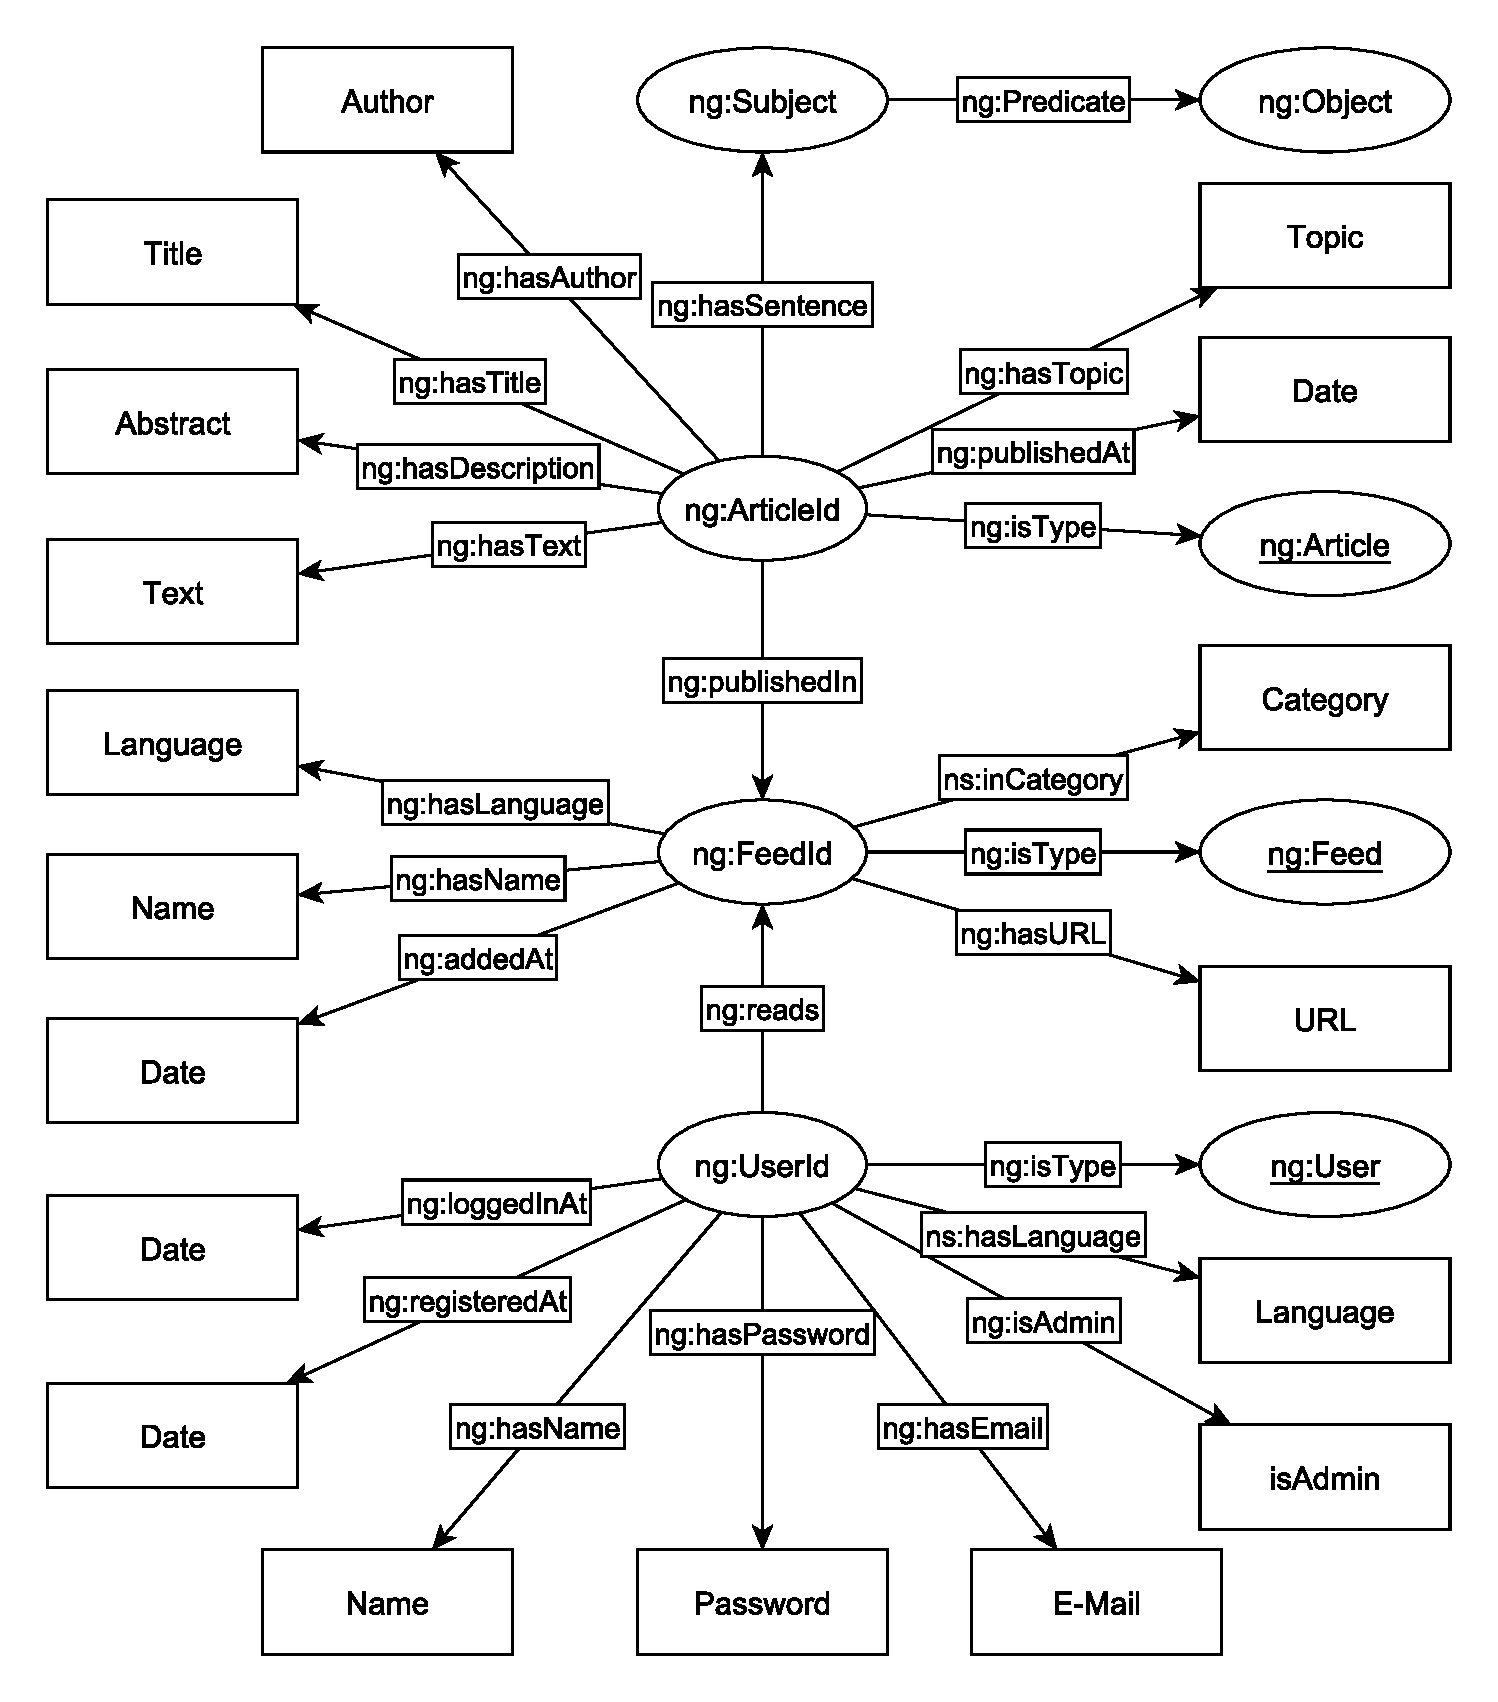
\includegraphics[width=0.90\textwidth]{Systementwurf/datenmodell/DBDiagramm.eps}
\caption{Datenbankdiagramm}
\label{fig:6.1}
\end{figure}
\section{Erläuterung}

Da wir einen Triplestore verwenden, gibt es keine wirklichen Entitäten und auch innerhalb der einzelnen Datensätze gibt es Verknüpfungen mit Kardinalität \( \neq\) 1. Die Kardinalitäten der Verknüpfungen innerhalb der Datensätze sind oben aufgeführt.

\begin{entity}{10}{User}
\begin{tabular}[ht]{|l|l|}
  \hline
  Beziehung & Kardinalität\\
  \hline
  reads & 0...n\\
  \hline
\end{tabular}
\end{entity}

\begin{entity}{20}{Artikel}
\begin{tabular}[ht]{|l|l|}
  \hline
  Beziehung & Kardinalität\\
  \hline
  publishedIn & 1\\
  \hline
  hasSentence & 0...n\\
  \hline
\end{tabular}
\end{entity}